\documentclass[]{article}

\usepackage[margin=1.0in]{geometry}
\usepackage{amsmath}
\usepackage{amsfonts}
\usepackage{amsthm}
\usepackage{graphicx}
\usepackage{amssymb}

\usepackage{mathtools}

\usepackage[
backend=bibtex,
style=alphabetic,
sorting=ynt
]{biblatex}
\addbibresource{refs}

\usepackage{hyperref}
\PassOptionsToPackage{hypernotes=false}{hyperref}

%opening
\title{Dirichlet Domains}
\author{Alex Karlovitz}
\date{}

\begin{document}
	
	\maketitle
	
In this note, we discuss the details involved in computing a Dirichlet domain for a group $\Gamma$ acting discretely on the upper half-plane model of hyperbolic 2-space.
As an example, we construct the compact arithmetic surface described by Kontorovich in \cite{kontorovich2011}.
	
\section*{Constructing a Dirichlet Domain}
	
To construct a Dirichlet domain, one starts with a specific point $z \in \mathbb{H}$ (we often take $z = 2i$).
Then, we find points in the orbit of $z$ under $\Gamma$ which are relatively close to $z$.
For each such point $z_*$, we find the geodesic of points which are equidistant from $z$ and $z^*$.
The set of points in $\mathbb{H}$ which are closer to $z$ than to any of the $z_*$'s will constitute a fundamental domain for $\Gamma\backslash\mathbb{H}$ so long as we took enough points in the orbit.

Here is pseudocode for finding the geodesic of points equidistant from two points $z_1$ and $z_2$ in $\mathbb{H}$.
\begin{verbatim}
def find_equidistant_geodesic(z1, z2) :
    # give names to real and imaginary parts for ease of reading
    x1, y1 = real(z1), imag(z1)
    x2, y2 = real(z2), imag(z2)

    # Step 1: get geodesic G through z1 and z2
    
    if x1 == x2 :
        # G is vertical line
        G = line((x1, 0), (x1, y1))
    else :
        # G is circle of center c and radius r
        c = (|z2|^2 - |z1|^2)/2/(x2 - x1)
        r = sqrt( (x1 - c)^2 + y1^2 )
        G = circle(c, r)
        
    # Step 2: get point z0 on G equidistant from z1 and z2 (in hyperbolic distance)
    
    eqn1 = |z - z1|^2/4/imag(z)/y1 == |z - z2|^2/4/imag(z)/y2
    if isCircle(G) :
        eqn2 = |z - c|^2 == r^2
    else :
        eqn2 = real(z) == x1
    z0 = solve((eqn1, eqn2), unknown=z)
    
    # Step 3: get geodesic G0 through z0 which meets G at a right angle
    
    x0, y0 = real(z0), imag(z0)
    if isCircle(G) :
        # first get slope of G at z0
        s = (c - x0)/y0
        
        # if the slope is 0, return vertical line through z0
        if s == 0 :
            return line((x0, 0), (x0, y0))
        
        # solve for center a and radius R
        a = -y0/s + x0
        R = sqrt( (x0 - a)^2 + y0^2 )
        
        G0 = circle(a, R)
    else :
        # z0 is at top of circle
        G0 = circle(x0, y0)
        
    return G0
\end{verbatim}

\section*{Cocompact Example}

In this section, we provide the details for applying Hejhal's algorithm to the compact arithmetic surface described in \cite{kontorovich2011}.
(We omit the details on where this surface comes from; see Kontorovich's note for a full discussion).
\\

In Figure \ref{FD}, we see the fundamental domain for this example.
\begin{figure}[h]
	\centering
	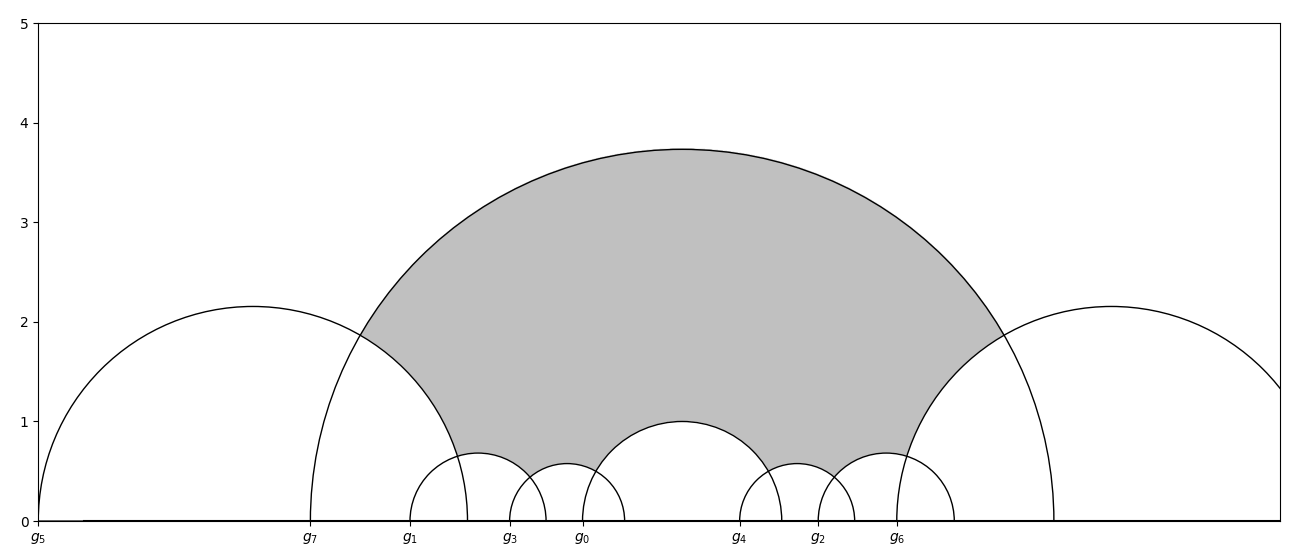
\includegraphics[width=\linewidth]{cocompact_fd.png}
	\caption{Fundamental domain for the compact arithmetic surface}
	\label{FD}
\end{figure}
The base point we used to produce this Dirichlet domain was $z = 2i$.
Next, we list the matrices $M_i$ which correspond to the geodesics $g_i$ in Figure \ref{FD}.
By this, we mean that $g_i$ is the geodesic of points in $\mathbb{H}$ equidistant from $z = 2i$ and $M_i(z)$.
\begin{align*}
	M_0 &= \begin{pmatrix}
		0 & -1 \\
		1 & 0
	\end{pmatrix} &
	M_1 &= \begin{pmatrix}
		-3 & 2 + 2\sqrt{3} \\
		-2 + 2\sqrt{3} & -3
	\end{pmatrix} &
	M_2 &= \begin{pmatrix}
		-3 & -2 - 2\sqrt{3} \\
		2 - 2\sqrt{3} & -3
	\end{pmatrix} &
	M_3 &= \begin{pmatrix}
		-2 & \sqrt{3} \\
		\sqrt{3} & -2
	\end{pmatrix} \\
	M_4 &= \begin{pmatrix}
		-2 & -\sqrt{3} \\
		-\sqrt{3} & -2
	\end{pmatrix} &
	M_5 &= \begin{pmatrix}
		-2 & 3 + 2\sqrt{3} \\
		-3 + 2\sqrt{3} & -2
	\end{pmatrix} &
	M_6 &= \begin{pmatrix}
		-2 & -3 - 2\sqrt{3} \\
		3 - 2\sqrt{3} & -2
	\end{pmatrix} &
	M_7 &= \begin{pmatrix}
		0 & -2 - \sqrt{3} \\
		2 - \sqrt{3} & 0
	\end{pmatrix}
\end{align*}
Let $\Gamma$ be the group generated by these matrices.
Noticing that some of these matrices are inverses of each other (recall that we are working in PSL$(2, \mathbb{R})$, so $MM^{-1} = \pm I$), we have that the group is generated by just five matrices
$$
\Gamma = \langle M_0, M_1, M_3, M_5, M_7 \rangle
$$
Next, observe that $M_i$ maps $g_j \mapsto g_i$ where $j$ is such that $M_j = M_i^{-1}$.
Moreover, $M_i$ maps the interior of $g_j$ (points closer to $M_j(z)$ than to $z$) to the exterior of $g_i$ (points closer to $z$ than to $M_i(z)$).
This suggests a straightforward pullback algorithm:
\begin{verbatim}
# z - a point in upper half space
# Ms - an ordering of all 8 matrices M_0, ..., M_7
#    in practice, we take Ms = [M0, M7, M3, M1, M5, M4, M2, M6]
def pullback(z, Ms) :
    for M in Ms :
        set g = geodesic corresponding to M
        if z in interior of g :
            z = M^(-1)(z)
            go back to start of for loop
            
    return z
\end{verbatim}
In words, we are simply checking every geodesic $g$ to see if $z$ is in the interior.
If it is, we apply $M^{-1}$ where $M$ is the matrix corresponding to $g$ then return to the beginning of the list.
If $z$ is in the exterior of every geodesic, then by definition it falls within the fundamental domain.
\\

Finally, note that
$$
-M_7M_0 =
\begin{pmatrix}
	2 + \sqrt{3} & 0 \\
	0 & 2 - \sqrt{3}
\end{pmatrix}
$$
In other words, $\Gamma$ \textit{already contains a nontrivial diagonal matrix}.
Therefore, our fundamental domain is already a flare domain, meaning we can apply Hejhal's algorithm without the need for any conjugation.

	\pagebreak
	
	\printbibliography
	
\end{document}